\chapter{Modelos de señal y muestras simuladas}
\label{ch:samples}
% \epigraph{\emph{“Champions keep playing until they get it right.”}}{Billie Jean King}


La simulación de los distintos procesos físicos bajo consideración y de la respuesta del detector es necesaria para optimizar y estimar el rendimiento de los distintos análisis. Además permite desarrollar las estrategias para la identificación de partículas antes de la toma de datos y comprobar la eficiencia de los algoritmos. La preparación de búsquedas de nueva física requiere una simulación detallada del detector para estimar su potencial de descubrimiento y desarrollar métodos óptimos para medir las propiedades de las partículas. Una correcta comprensión de los eventos de señal y fondo es esencial para distinguir entre ambos. Una vez que se dispone de datos de colisiones reales, también se necesitan datos simulados para encontrar desviaciones de \ac{SM}. Todos los pasos de la simulación \ac{MC} se describieron en \Sect{\ref{sec:theory:mc_simulation}}.

De forma similar a cualquier análisis de física en el \ac{LHC}, este análisis hace uso de muestras simuladas, tanto para entender las posibles señales a descubrir, como para hacer un modelado correcto del fondo con estados finales de \gammajet.
En este capítulo se dan detalles sobre la generación y simulación de las muestras de señal y fondo.


\section{Señales}
\label{sec:samples:samples:sig}

\subsection{Quarks excitados}
\label{subsec:samples:samples:sig:qstar}

Una de las dos teorías que se ponen a prueba en esta tesis corresponde a la de \acf{EQ}, que se explicó detalladamente en la \Sect{\ref{subsec:theory:bsm:qstar}}. Si los quarks en realidad están compuestos por constituyentes más fundamentales unidos entre sí por alguna interacción desconocida, deberían aparecer nuevos efectos dependiendo del valor de la escala de composición \(\Lambda\).
También se vio que los \acp{EQ} se acoplan a los bosones del \ac{SM}, cuyas fuerzas están determinadas por las constantes de acoplamiento \(f\), \(f'\) y \(f_s\).

En esta teoría, hay un total de 5 parámetros: la escala de composición \(\Lambda\), los tres acoplamientos y la masa del \ac{EQ}. Para reducir el número de parámetros, es habitual fijar \(\Lambda = \mq\)~\cite{Zhan_Li_Liu_Li-2016}, y tomar las tres constantes de acoplamiento como iguales. De esta manera, sólo la masa y el acoplamiento son los parámetros libres de la teoría.

Se producen muestras de eventos de \ac{EQ} utilizando el software \pythia 8.245~\cite{Pythia8.2} con el conjunto de \acp{PDF1} a \ac{LO} de NNPDF 2.3~\cite{NNPDF2} y el tune A14 para el \ac{UE}.
Por primera vez en los estados finales de \gammajet en el \ac{LHC}, se consideran tres sabores diferentes: \ac{EQ} livianos (o light) \qstar (\(u^* / d^*\)) y pesados, separando entre \cstar y \bstar. Además, en este trabajo se estudian diferentes acoplamientos con los siguientes valores: \(f = 0.01, \, 0.1, \, 0.5, \, 0.75, \, 1.0\). Las masas de los \acp{EQ} y los acoplamientos utilizados se enumeran en la \Tab{\ref{tab:samples:samples:sig:qstar:xs}} donde se muestra la sección eficaz de los eventos multiplicada por el \textit{branching ratio}. Además, todos estos valores se muestran en la \Fig{\ref{tab:samples:samples:sig:qstar:xs}}.



\begin{table}[ht!]
    \centering
    \caption{Producto de la sección eficaz y el branching ratio en fb del modelo de \acp{EQ} para los tres sabores considerados y las distintas constantes de acomplamiento.}
    \resizebox{\linewidth}{!}{
        \begin{tabular}{lcccccc}
            \toprule
            \multirow{2}{*}{Quark excitado}  & \multirow{2}{*}{Masa [GeV]}  
            & \multicolumn{5}{c}{Acoplamiento \(f=f'=f_s\)}
            \\
            \cmidrule(l){3-7}
            &           & 0.01          & 0.10      & 0.50          & 0.75      & 1.00          \\
            \midrule
            \multirow{10}{*}{\(\qstar \rightarrow \gamma + u/d\)}
            & $500$     & 29.9400       & 3007.0000 & 75240.0000    & -         & 304200.0000   \\
            & $1000$    & 1.6560        & 165.0000  & 4153.0000     & -         & 16490.0000    \\
            & $2000$    & 0.0536        & 5.3800    & 133.2000      & -         & 520.8000      \\
            & $3000$    & -             & 0.4435    & 11.0200       & -         & 43.0600       \\
            & $4000$    & -             & 0.0488    & 1.2270        & -         & 4.8240        \\
            & $5000$    & -             & -         & 0.1450        & -         & 0.5877        \\
            & $5500$    & -             & -         & -             & -         & 0.2064        \\
            & $6000$    & -             & -         & 0.0163        & 0.0384    & 0.0719        \\
            & $6500$    & -             & -         & -             & -         & 0.0250        \\
            & $7000$    & -             & -         & -             & 0.0043    & 0.0088        \\
            \midrule
            \multirow{5}{*}{\(\cstar \rightarrow \gamma + c\)}
            & $500$     & 3.6540        & 362.2000  & 9051.0000     & -         & 36290.0000    \\
            & $1000$    & 0.1333        & 13.3400   & 332.4000      & -         & 1297.0000     \\
            & $2000$    & -             & 0.2434    & 6.0190        & -         & 23.6800       \\
            & $3000$    & -             & -         & 0.3135        & -         & 1.2450        \\
            & $4000$    & -             & -         & -             & -         & 0.0906        \\
            \midrule
            \multirow{5}{*}{\(\bstar \rightarrow \gamma + b\)}
            & $500$     & 0.6381        & 63.7700   & 1588.0000     & -         & 6324.0000     \\
            & $1000$    & 0.0220        & 2.2080    & 54.7600       & -         & 215.4000      \\
            & $2000$    & -             & 0.0372    & 0.9249        & -         & 3.6200        \\
            & $3000$    & -             & -         & 0.0446        & -         & 0.1770        \\
            & $4000$    & -             & -         & -             & -         & 0.0121        \\
            \bottomrule
        \end{tabular}
    }
    \label{tab:samples:samples:sig:qstar:xs}
\end{table}

\begin{figure}[ht!]
    \centering
    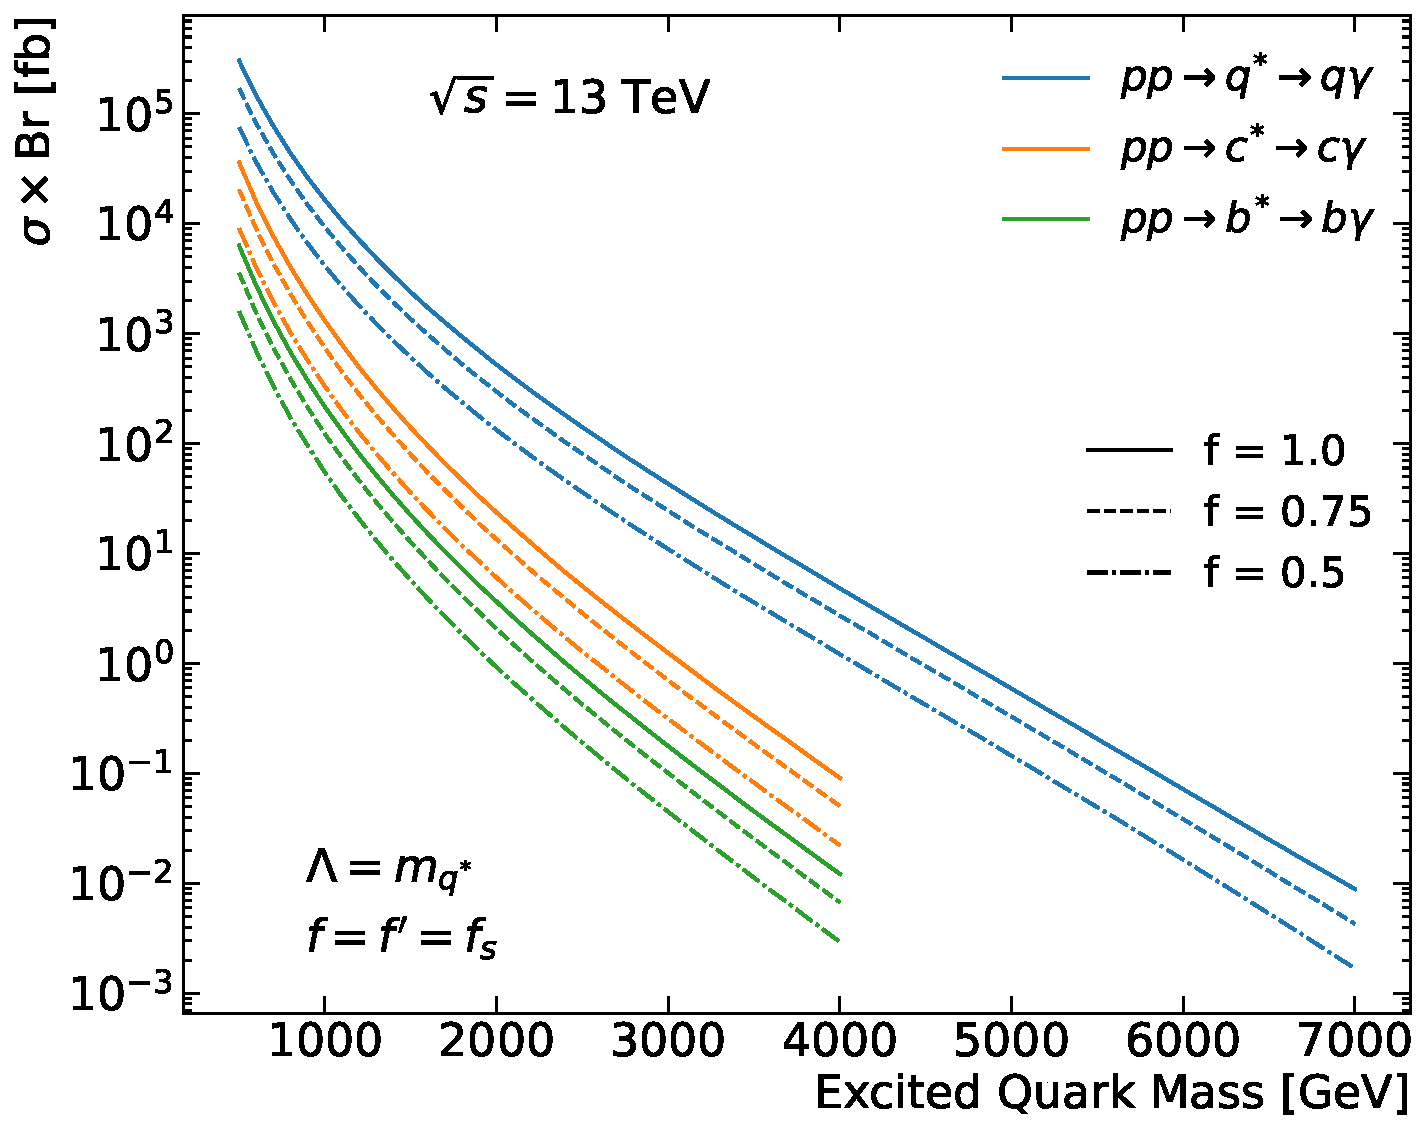
\includegraphics[width=0.6\linewidth]{5_resonances/samples/qstar_xs}
    \caption{Producto de la sección eficaz y el branching ratio de los diferentes modos de producción de los \acp{EQ} como función de la masa del \ac{EQ} a una energía de centro de masa de \(\sqs=13~\tev\). La figura muestra la comparación entre las señales de \qstar (azul), \cstar (naranja) y \bstar (verde) utilizando los acoplamientos de \(f=1.0,\, 0.75,\, 0.5\).}
    \label{fig:samples:samples:sig:qstar:xs}
\end{figure}


% Finalmente, en la \Fig{\ref{fig:samples:samples:sig:qstar:couplings}}, se muestra una comparación entre dos eñales de \qstar con diferentes acoplamientos.
% \begin{figure}[ht!]
%     \centering
%     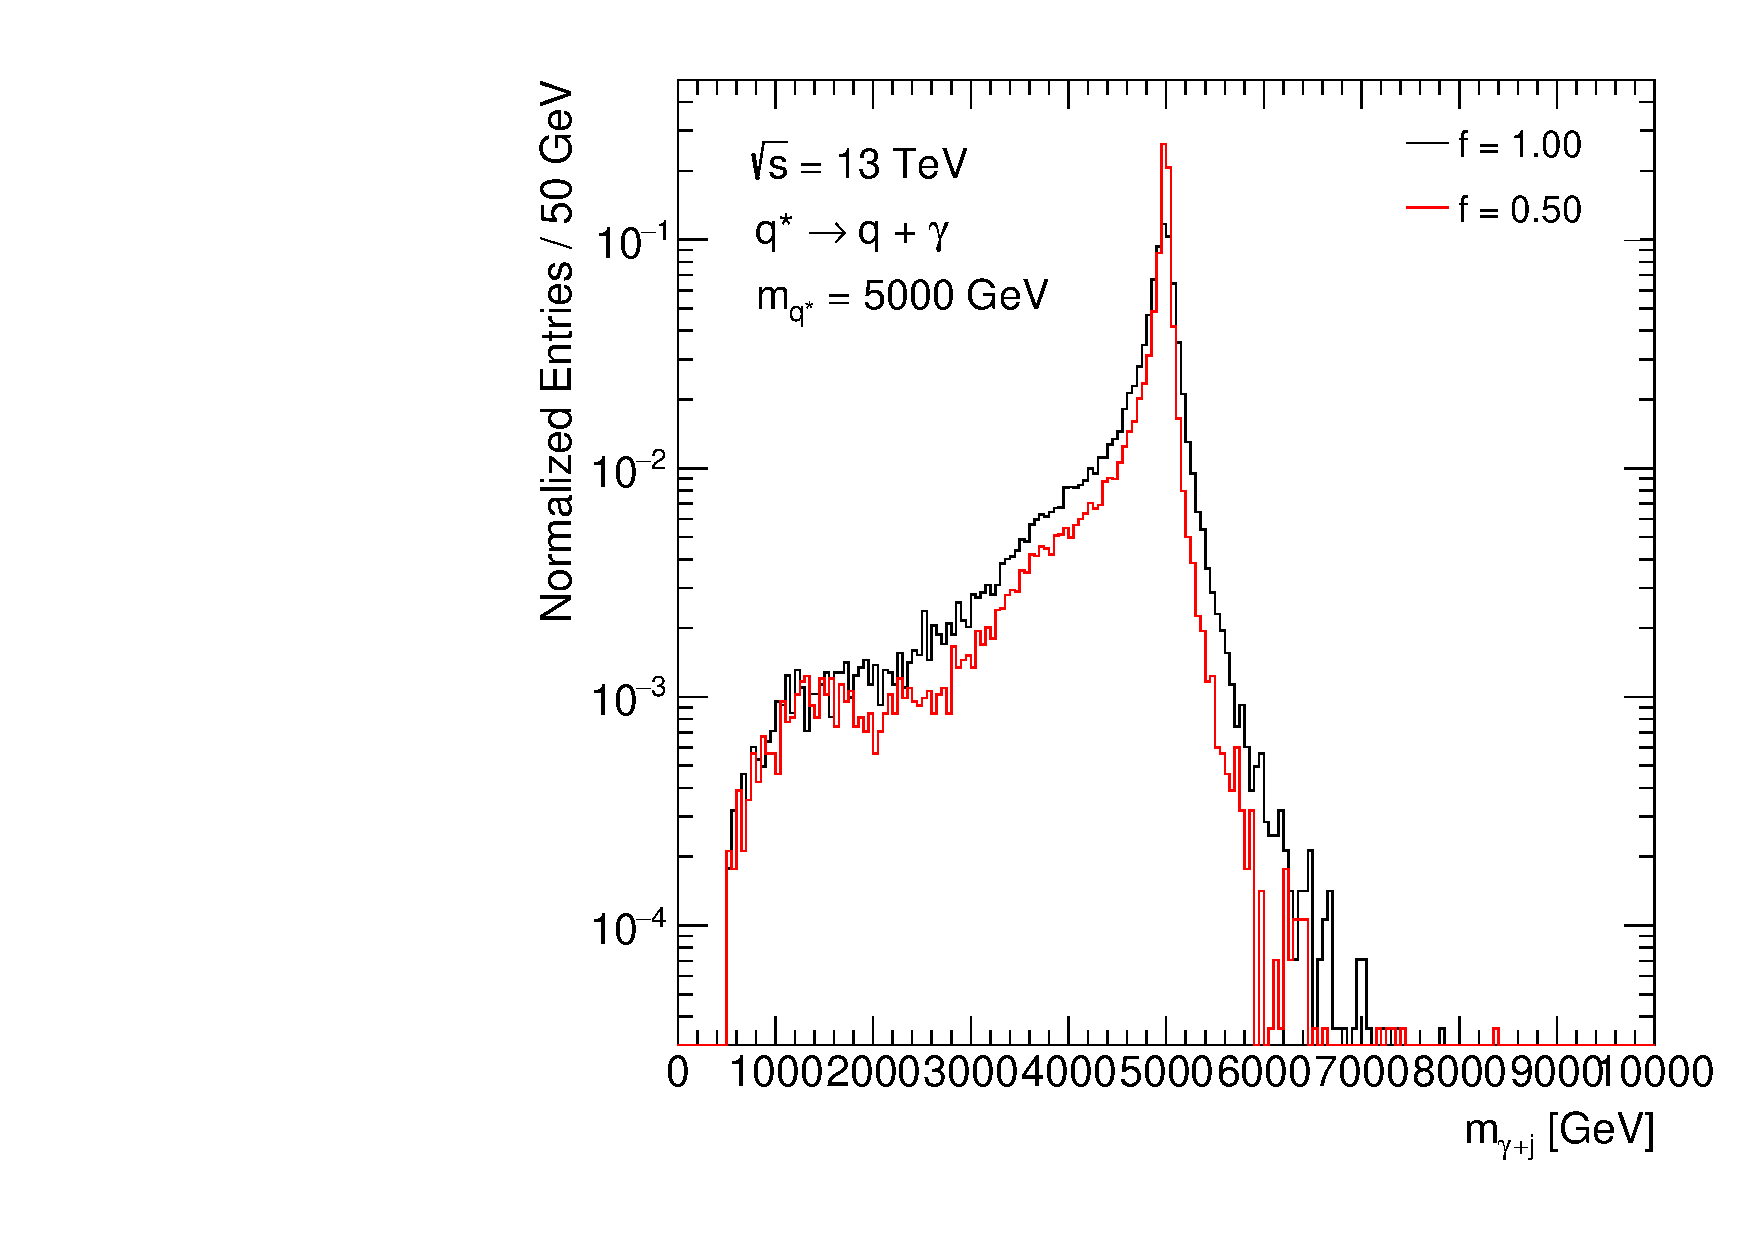
\includegraphics[width=0.5\linewidth]{5_resonances/samples/qstar/couplings}
%     \caption{Comparación de dos señales de \qstar con masa \(\mq=5000~\gev\) utilizando diferentes acoplamientos: \(f=1.00\) (negro) y \(f=0.50\) (rojo).}
%     \label{fig:samples:samples:sig:qstar:couplings}
% \end{figure}




\subsection{Micro-Agujeros Negros}
\label{subsec:samples:samples:sig:qbh}

% La producción de \ac{QBH} en colisiones \pp del \ac{LHC} es predicha por modelos con dimensiones extra.

A través de la existencia de dimensiones extra, se predice la producción de \acf{QBH} en el \ac{LHC}, en colisiones \pp.
La sección eficaz de producción viene determinada por el radio gravitatorio que depende de la escala de Planck y del número de dimensiones, formulada como una sección eficaz clásica.


Las muestras de \ac{QBH} que decaen en un fotón y un partón se generan con el software \ac{QBH} 3.01 descripto en la \Refn{\cite{QBH}} y \pythia 8.3 para la hadronización y el \ac{UE}. Se ha utilizado el conjunto de \acp{PDF1} CTEQ6L1 junto con el tune estándar A14 del \ac{UE}. Para la generación de los eventos, se fija el rango de masa de producción de agujeros negros desde la escala de Planck \(m_p\) a \(3 m_p\) o la energía del centro de masa \sqs, la que sea menor. Se tienen en cuenta dos modelos diferentes, en función del número de dimensiones adicionales \(n\). El modelo ADD, como se discute en la \Sect{\ref{subsec:theory:bsm:qbh}}, considera 6 dimensiones extra, lo que lleva a un número total de 10 dimensiones espacio-temporales. Por otro lado, el modelo RS1 propone sólo una dimensión extra deformada. Dado que para este análisis sólo interesa el estado final de \gammajet, se consideran los 6 estados no térmicos de agujero negro que se muestran en la \Sect{\ref{subsec:theory:bsm:qbh}}. Las secciones eficaces multiplicadas por el branching ratio de los dos modelos se representan en la \Fig{\ref{fig:samples:samples:sig:qbh:xs}} y los valores correspondientes en la \Tab{\ref{tab:samples:samples:sig:qbh:xs}}.


\begin{figure}[ht!]
    \centering
    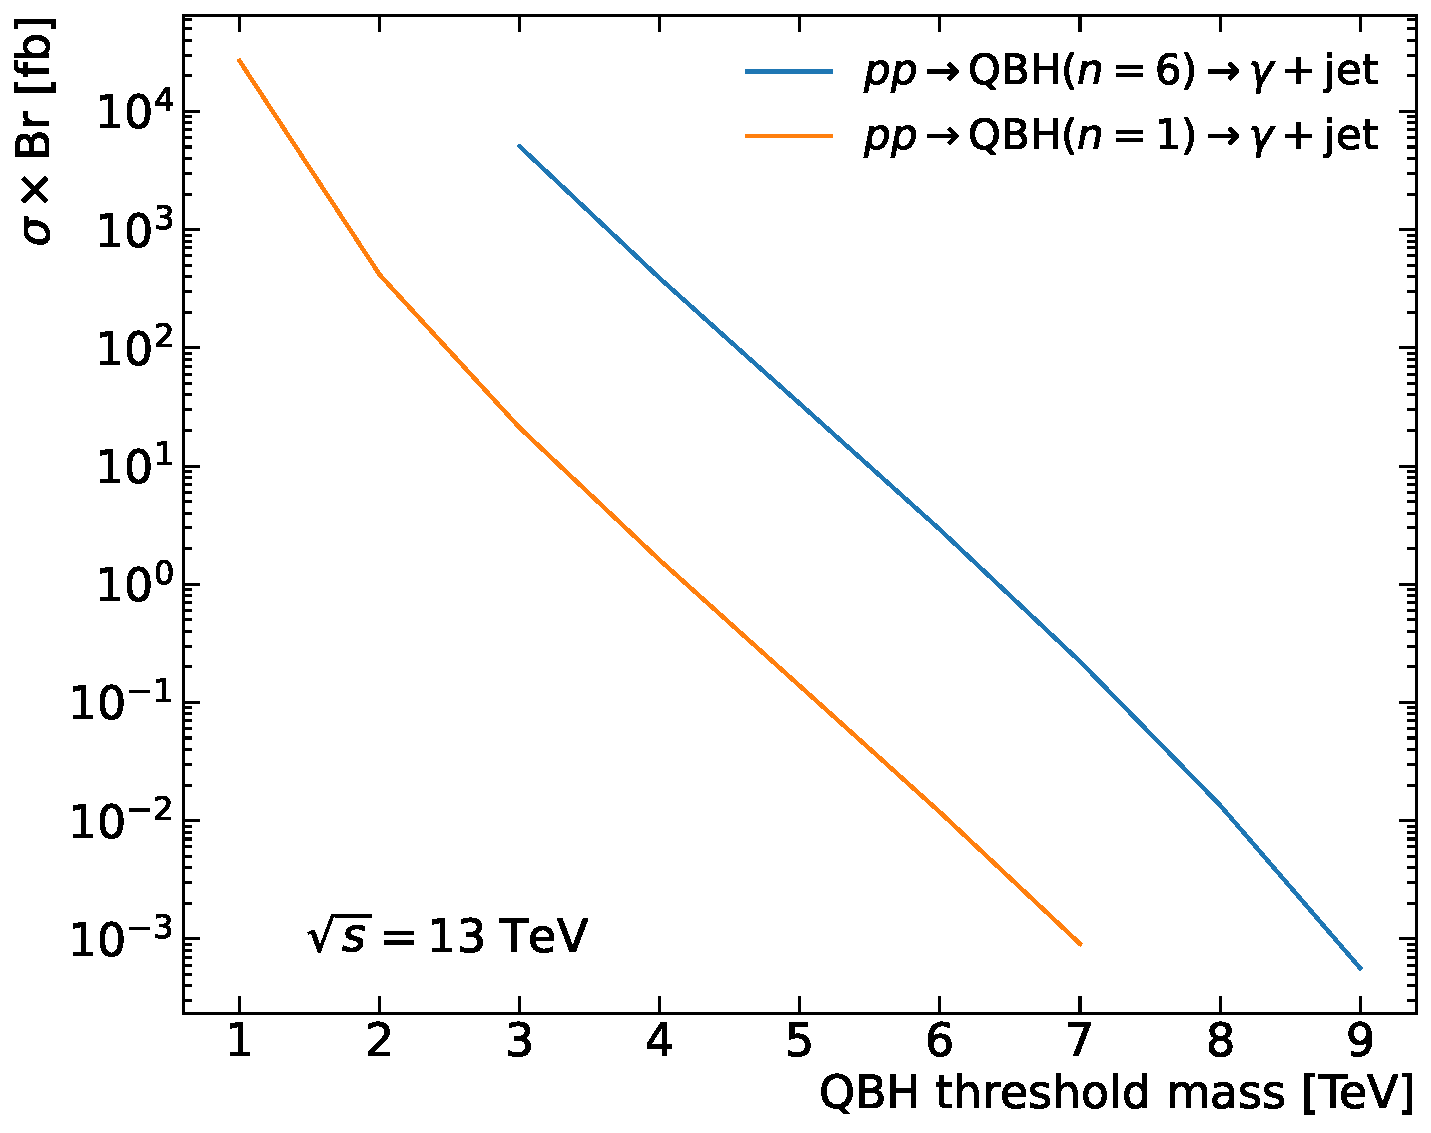
\includegraphics[width=0.6\linewidth]{5_resonances/samples/qbh_xs}
    \caption{Producto de la sección eficaz y el branching ratio para los modelos RS1 (naranja) y ADD (azul) de \ac{QBH} para una energía de centro de masa de \(\sqs=13~\tev\).}
    \label{fig:samples:samples:sig:qbh:xs}
\end{figure}


\begin{table}[ht!]
    \caption{Suma de productos de sección eficaz y branching ratio en fb para los seis estados no termales de los \acp{QBH} que decaen en un par \gammajet.}
    \begin{center}
        \begin{tabular}{ccc}
            \toprule
            \mqbh [GeV] & ADD (\(n=6\))         & RS1 (\(n=1\)) \\
            \midrule
            1000        &                       & $2.69\times 10^{+4}$  \\
            2000        &                       & $4.17\times 10^{+2}$  \\
            3000        & $5.07\times 10^{+3}$  & $2.11\times 10^{+1}$  \\
            4000        & $3.88\times 10^{+2}$  & $1.60\times 10^{+0}$  \\
            5000        & $3.37\times 10^{+1}$  & $1.38\times 10^{-1}$  \\
            6000        & $2.90\times 10^{+0}$  & $1.18\times 10^{-2}$  \\
            7000        & $2.22\times 10^{-1}$  & $9.08\times 10^{-4}$  \\
            8000        & $1.35\times 10^{-2}$  &                       \\
            9000        & $5.64\times 10^{-4}$  &                       \\
            \bottomrule
        \end{tabular}
    \end{center}
    \label{tab:samples:samples:sig:qbh:xs}
\end{table}












\section{Fondos del SM}
\label{sec:samples:samples:bkg}


En el estado final de interés en el que hay al menos un fotón y un jet, la producción de fotones prompt de \ac{QCD} es el principal proceso del \ac{SM} que no puede reducirse.
Para estudiar esta particular contribución del fondo, se utilizan las muestras de \ac{MC}.
Además, existe una fracción considerable de eventos de dijet en los cuales un jet es mal-identificado como un fotón, teniendo entonces una contribución adicional al fondo. Para estudiar esta contribución en particular se ha utilizado un enfoque basado en datos que se describe en el \Ch{\ref{ch:bkg}}.


Se generan muestras con un gran número de eventos de \gammajet utilizando el software \Pythia 8.186~\cite{Pythia8.1}. Los procesos partónicos se simulan usando \ac{ME} a \ac{LO} con la inclusión de lluvias de partones de estado inicial y final, donde la parametrización de la estructura del protón viene dada por la \acp{PDF1} a \ac{LO} de \texttt{NNPDF2.3}~\cite{NNPDF2}.
El proceso de hadronización se modela mediante el modelo de cuerdas de Lund~\cite{Anderson-1983}, brevemente discutido en la \Sect{\ref{subsec:theory:mc_simulation:hadronisation}}, y la muestra también cuenta con una simulación del \ac{UE}.
Los parámetros del generador de eventos se ajustan según el tune A14 para \Pythia~\cite{Pythia-A14Tune}.
La muestra \pythia, dado que se genera a \ac{LO}, permite la separación entre las contribuciones de fotones directos y de fragmentación (véase la \Sect{\ref{subsec:theory:sm:prompt_photon}}).

Se consideran un conjuntos de muestras con diferentes umbrales de \pt a fin de optimizar la generación de los eventos. Los detalles de cada muestra, incluida la sección eficaz y las eficiencias de los filtros, se muestran en la \Tab{\ref{tab:samples:samples:bkg:samples}}.

\begin{table}[ht!]
    \caption{Detalles de las muestras simuladas del fondo de \gammajet.}
    \centering
    \resizebox{\textwidth}{!}{
        \begin{tabular}{l c l r r}
            \toprule
            Nombre de la muestra      &  Nombre del generador                  &   División de \pt [GeV]    & Sección eficaz [pb] &  Eficiencia del filtro  \\
            \midrule
            \gammajet direct &  \Pythia 8.244.3+\EvtGen v.1.7.0 &  \([70, 140]\)        & 28396.0           &  7.2863E-02   \\
            \gammajet direct &  \Pythia 8.244.3+\EvtGen v.1.7.0 &  \([140, 280]\)       & 2625.5            &  7.0598E-02   \\
            \gammajet direct &  \Pythia 8.244.3+\EvtGen v.1.7.0 &  \([280, 500]\)       & 198.39            &  6.0369E-02   \\
            \gammajet direct &  \Pythia 8.244.3+\EvtGen v.1.7.0 &  \([500, 800]\)       & 18.846            &  4.4596E-02   \\
            \gammajet direct &  \Pythia 8.244.3+\EvtGen v.1.7.0 &  \([800, 1000]\)      & 2.3312            &  2.4130E-02   \\
            \gammajet direct &  \Pythia 8.244.3+\EvtGen v.1.7.0 &  \([1000, 1500]\)     & 0.79945           &  2.3667E-02   \\
            \gammajet direct &  \Pythia 8.244.3+\EvtGen v.1.7.0 &  \([1500, 2000]\)     & 0.055512          &  1.9632E-02   \\
            \gammajet direct &  \Pythia 8.244.3+\EvtGen v.1.7.0 &  \([2000, 2500]\)     & 0.0052361         &  1.6644E-02   \\
            \gammajet direct &  \Pythia 8.244.3+\EvtGen v.1.7.0 &  \([2500, 3000]\)     & 0.00052733        &  1.4446E-02   \\
            \gammajet direct &  \Pythia 8.244.3+\EvtGen v.1.7.0 &  \([3000, \infty]\)   & 4.8856e-05        &  1.4371E-02   \\
            \gammajet frag   &  \Pythia 8.244.3+\EvtGen v.1.7.0 &  \([70, 140]\)        & 106180000.0       &  1.9271E-05   \\
            \gammajet frag   &  \Pythia 8.244.3+\EvtGen v.1.7.0 &  \([140, 280]\)       & 6702000.0         &  2.0959E-05   \\
            \gammajet frag   &  \Pythia 8.244.3+\EvtGen v.1.7.0 &  \([280, 500]\)       & 344070.0          &  2.0507E-05   \\
            \gammajet frag   &  \Pythia 8.244.3+\EvtGen v.1.7.0 &  \([500, 800]\)       & 23711.0           &  1.6991E-05   \\
            \gammajet frag   &  \Pythia 8.244.3+\EvtGen v.1.7.0 &  \([800, 1000]\)      & 2284.6            &  1.0123E-05   \\
            \gammajet frag   &  \Pythia 8.244.3+\EvtGen v.1.7.0 &  \([1000, 1500]\)     & 701.22            &  1.0074E-05   \\
            \gammajet frag   &  \Pythia 8.244.3+\EvtGen v.1.7.0 &  \([1500, 2000]\)     & 70.086            &  5.0238E-06   \\
            \gammajet frag   &  \Pythia 8.244.3+\EvtGen v.1.7.0 &  \([2000, \infty]\)   & 11.548            &  2.4464E-06   \\
            \bottomrule
        \end{tabular}
    }
    \label{tab:samples:samples:bkg:samples}
\end{table}

Como se mencionó más arriba, el fondo de las muestras de datos finales se estima a partir de los propios datos utilizando diferentes formas funcionales. Las muestras simuladas del fondo, no obstante, son de gran utilidad para el proceso de optimización de las regiones de señal (\Ch{\ref{ch:evt_selection}}) así como para la selección de las formas funcionales que se ajustará a los datos, como se verá en la \Sect{\ref{sec:bkg:modeling}}.